O SAD SustenAgro (capítulo \ref{chap:SustenAgro}) foi instanciado
usando o Framework Decisioner (capítulo \ref{chap:Decisioner}) e
avaliado, durante diferentes estágios de desenvolvimento, através
de experimentos realizados com especialistas de domínio e usuários
da Embrapa. Esses dois sistemas foram desenvolvidos com metodologias
iterativas, onde foram realizadas varias inspeções e testes durante
a implementação. Uma avaliação final também foi realizada para analisar
se as funcionalidades foram implementadas corretamente.

A seguir, são apresentadas as avaliações realizadas no SAD SustenAgro
e ao Framework Decisioner. Elas foram independentes e geraram resultados
que levaram ao redesenho das arquiteturas de ambos sistemas em diferentes
etapas do seu desenvolvimento.

\section{Avaliação das Web UI.}

Na finalização do processo de design das Web UI, explicado na Seção
\ref{sec:Web-UI}, foi realizada uma avaliação da usabilidade das
mesmas no SAD SustenAgro. Os detalhes dessa avaliação foram:
\begin{description}
\item [{Data}] Junho de 2015
\item [{Participantes}] Usuários da ferramenta: especialista em sustentabilidade
e especialista em economia agrícola
\item [{Local}] Instituto de Ciências Matemáticas e de Computação (ICMC-USP)\nomenclature{ICMC}{ Instituto de Ciências Matemáticas e de Computação} 
\item [{Técnica}] Avaliação de usabilidade
\end{description}
Nesta avaliação foi apresentado, aos usuários especialistas em sustentabilidade,
o processo de design da UI e o protótipo da interface gráfica de usuário
do SAD SustenAgro sem dados reais. Nessas interfaces, eles interagiram
com as telas, através de um navegador web, fazendo uso das funcionalidades
do SAD que simulava os dados durante o processo.

Durante esta avaliação foram verificados, os três aspectos da usabilidade:
\begin{itemize}
\item Eficácia: as interfaces permitiram realizar as tarefas segundo as
funcionalidades definidas e permitiam interagir de maneira intuitiva
para realizar as tarefas.
\item Eficiência: o aceso à ferramenta foi realizado em tempos esperados
e foi possível realizar as tarefas com recursos típicos de um laptop
e um navegador web.
\item Satisfação: os usuários conseguiram realizar as tarefas sem problemas
e com uma experiência de fácil uso, onde a ferramenta fornecia informação
de ajuda para realizar as interações.
\end{itemize}
A avaliação foi positiva, cumprindo os três requisitos anteriores
de usabilidade. Esta avaliação gerou várias recomendações para melhorar
a interface gráfica de usuário, entre elas as mais relevantes foram: 
\begin{itemize}
\item Mudar a organização do processo de avaliação, agrupando varias tarefas
em uma seção denominada ``caracterização da unidade produtiva'',
que permite definir a localização, as principais características e
a disponibilização da informação em um processo unificado. 
\item Agrupar os resultados em uma seção ``Resultados'', integrando os
\foreignlanguage{english}{Web Components} específicos do SustenAgro
com os resultados da avaliação.
\item Organizar os indicadores em uma hierarquia simplificada que facilita
o preenchimento dos mesmos.
\end{itemize}
Depois de implementar as recomendações anteriores, foi continuado
o desenvolvimento com a integração da ontologia SustenAgro e da DSL.
Foi necessário realizar ajustes da interface ao integrar cada funcionalidade.
As principais mudanças foram realizadas devido a esta avaliação.

\section{Avaliação da ontologia de domínio de avaliação da sustentabilidade.}

A ontologia SustenAgro foi o resultado da modelagem do conhecimento
dos especialistas, que passou por várias etapas, desde ser definida
em texto, modelada em mapas conceituas e criada a ontologia em \foreignlanguage{english}{OWL}
(esse processo foi detalhado na Seção \ref{sec:Metodologia}). Cada
uma dessas etapas requereu inspeções por parte dos especialistas para
verificar a correta modelagem, uma avaliação formal foi realizada
e os detalhes são descritos a seguir.
\begin{description}
\item [{Data}] 14 de abril do 2016
\item [{Participantes}] Especialista em sustentabilidade e especialista
em modelagem de conhecimento
\item [{Local}] Embrapa Informática Agropecuária - Campinas
\item [{Técnica}] Visualização da ontologia e recuperação de conhecimento
\end{description}
O especialista em modelagem de conhecimento da Embrapa Informática
Agropecuária e o especialista em sustentabilidade reuniram-se para
realizar a revisão da ontologia SustenAgro por meio de ferramentas
de engenharia de conhecimento que permitiram visualizar as ontologias.

As ferramentas usadas na avaliação foram yWorks \footnote{\url{http://www.yworks.com/}}
e Gephi \footnote{\url{https://gephi.org/}}. Elas representaram aspectos
da ontologia usando diversas visualizações de grafos, permitindo avaliar
a coerência das conexões entre os nós daqueles grafos.

Também foi analisado o SAD SustenAgro, que tinha a ontologia integrada,
usando as funcionalidades que requeriam dados da ontologia, verificando
a informação recuperada e a coerência dela em relação à existente
na ontologia. 

A reunião de avaliação chegou no consenso: a ontologia \foreignlanguage{english}{OWL}
está representando a avaliação da sustentabilidade do sistema de produção
de cana no centro-sul do Brasil, destacando a especificidade dela
para suportar o SAD Sustenagro e que seu foco em conceitos concretos.

Foi recomendado integrar outros tipos de visualizações e editores
de ontologia no framework Decisioner. Entre eles foi recomendado fornecer
um editor visual de ontologias, basado na ferramenta \foreignlanguage{english}{WebVOWL,}
definida e desenvolvida por \citet{lohmann2014webvowl}. Devido a
limitações de tempo, não foi possível a implementação dessa sugestão
específica.

\section{Avaliação do protótipo funcional com dados}

Com a finalidade de avaliar a implementação do método SustenAgro,
foram realizados testes de vários tipos de avaliações, para comparar
com resultados de outras fontes, e assim validar a correta implementação.
Os detalhes da avaliação foram.
\begin{description}
\item [{Data}] 6 de junho do 2016
\item [{Participantes}] Especialista em sustentabilidade e especialista
em economia agrícola
\item [{Local}] Agência Paulista de Tecnologia dos Agronegócios (APTA)
\item [{Técnica}] Testes numéricos dos resultados do software
\end{description}
A revisão dos resultados numéricos foi realizada a partir de vários
cenários de indicadores, sendo realizada uma comparação dos resultados
processados manualmente com os resultados de avaliação do SAD SustenAgro.
Os resultados manuais foram iguais aos calculados pelo sistema, o
que permitiu validar a correta definição do método SustenAgro e sua
implementação no SAD SustenAgro. 

Os cenários avaliados foram casos extremos dos indicadores, processo
denominado teste de mínimos e máximos, gerando resultados em forma
de relatório para cada um dos cenários. A Figura \ref{fig:Matriz-de-sustentabilidade-Maximos}
apresenta a Matriz de Sustentabilidade com o cenário de mínimos, na
qual o ponto preto identifica o resultado da avaliação. Ele ficou
no primeiro quadrante tal como se esperava. Os resultados para testes
de máximos também se comportaram como esperado.

\begin{figure}[H]
\begin{centering}
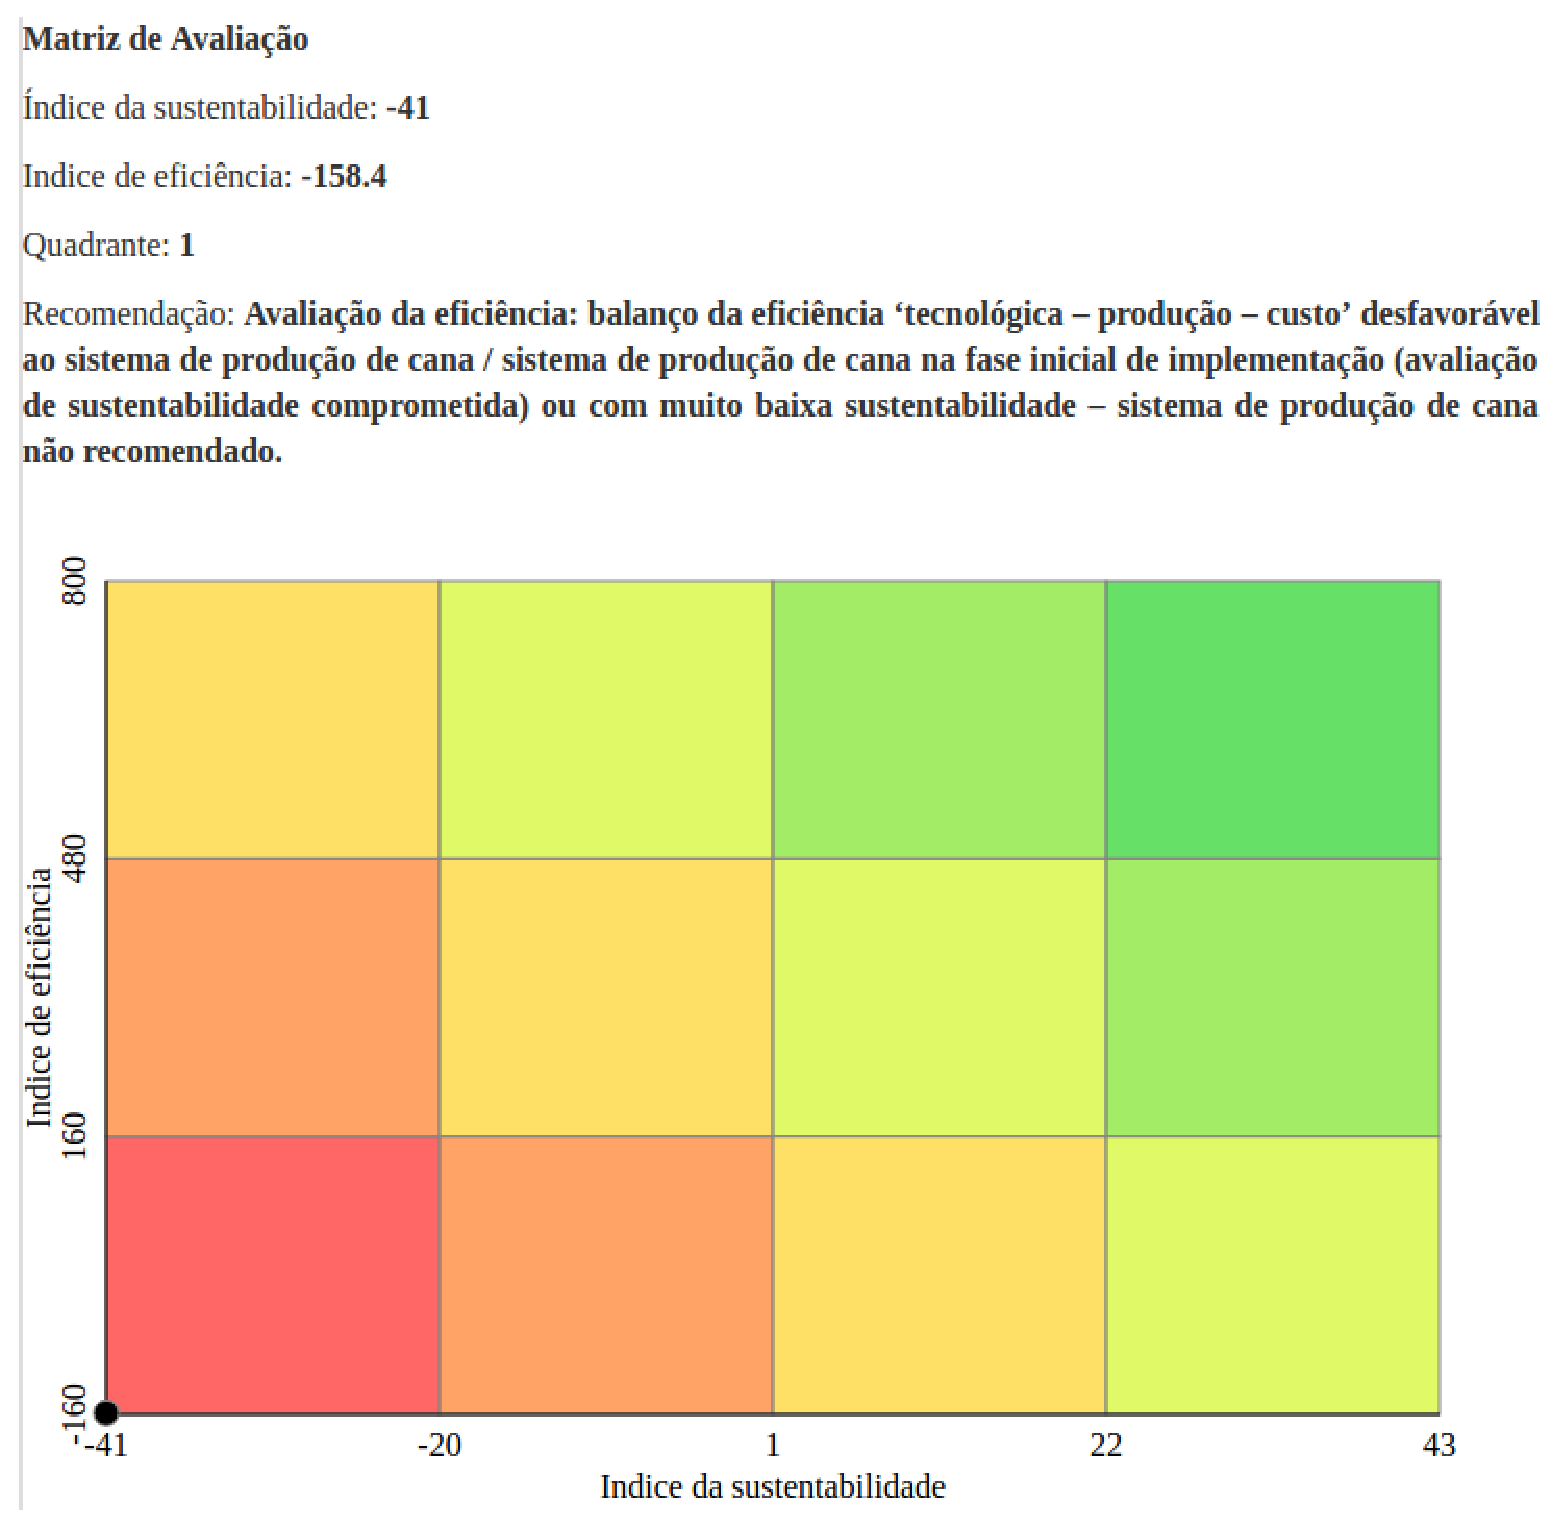
\includegraphics[width=0.8\columnwidth]{figures/Minimum}
\par\end{centering}
\caption{Matriz de Sustentabilidade com valores mínimos.\label{fig:Matriz-de-sustentabilidade-Maximos}}

\end{figure}

Um dos aspectos importantes da ferramenta, é que ela permite que os
próprios especialistas mudem, em tempo real, as fórmulas do método
de avaliação, permitindo fazer ajustes finos no método. Essa funcionalidade
permitiu descobrir e avaliar rapidamente um problema do método original:
a integração de uma operação de valor de um valor absoluto na fórmula.
A possibilidade da interação direta e fácil dos especialistas, em
tempo real, com o sistema permitiu demostrar agilmente possíveis cenários
de resolução do problema e aceitar rapidamente uma solução, proposta
pelo autor.

\section{Avaliação do SAD SustenAgro e do Framework Decisioner: }

A partir da avaliação da ontologia, da implementação do método SustenAgro
e do desenvolvimento das Web UI realizou-se uma avaliação do SAD com
a finalidade de avaliar a integração desses componentes.
\begin{description}
\item [{Data}] 18 de maio do 2016 até o dia 22 de junho do 2016
\item [{Participantes}] Usuários especialistas e usuários finais.
\item [{Local}] Instituto de Ciências Matemáticas e de Computação (ICMC-USP)
\item [{Técnica}] Teste de usabilidade
\end{description}
Para realizar uma avaliação integral do SAD SustenAgro e do Framework
Decisioner, foi necessário fazer testes de usabilidade com usuários
de ambos os perfis do sistema (especialistas de domínio e usuários
finais). Essa avaliação foi realizada com a maioria dos membros da
equipe SustenAgro e com usuários finais, de maneira remota e independente,
totalizando 8 avaliações.

A avaliação consistiu em realizar um conjunto de tarefas com o SAD
SustenAgro v1.0 e responder se foi possível terminar a tarefa e as
sugestões. As tarefas e perguntas solicitadas aos usuários estão listadas
no Apêndice \ref{sec:Formul=0000E1rio-de-avalia=0000E7=0000E3o-SustenAgro}
e permitiram gerar os seguintes resultados das avaliações:

\begin{longtable}{|>{\centering}p{0.2\columnwidth}|>{\centering}p{0.2\columnwidth}|>{\centering}p{0.6\columnwidth}|}
\hline 
\textbf{\small{}Perfil de Usuário} & \textbf{\small{}Avaliação} & \textbf{\small{}Sugestões}\tabularnewline
\hline 
\hline 
{\small{}Usuário final 1} & {\small{}Positiva, realizou as 5 tarefas de usuário final com sucesso} & \begin{itemize}
\item {\small{}Aumentar a ajuda para cada funcionalidade}{\small \par}
\item {\small{}Barra de progresso durante a avaliação}{\small \par}
\item {\small{}Resultados de avaliação mais detalhados}
\end{itemize}
\tabularnewline
\hline 
\hline 
{\small{}Usuário final 2} & {\small{}Positiva, realizou as 5 tarefas de usuário final com sucesso} & \begin{itemize}
\item {\small{}Melhorar a explicação do processo de avaliação}{\small \par}
\item {\small{}Resultados numéricos com formatação }
\end{itemize}
\tabularnewline
\hline 
\hline 
{\small{}Usuário final 3} & {\small{}Positiva, realizou as 5 tarefas de usuário final com sucesso} & \begin{itemize}
\item {\small{}Segurança no cadastro da senha}{\small \par}
\item {\small{}Melhorar a localização do botão avaliar}{\small \par}
\item {\small{}Remover }\foreignlanguage{english}{{\small{}scroll}}{\small{}
externo}{\small \par}
\item {\small{}Salvar automaticamente os dados}
\end{itemize}
\tabularnewline
\hline 
\hline 
{\small{}Especialista em sustentabilidade} & {\small{}Positiva, realizou as 5 tarefas de usuário e as 5 tarefas
de especialista de domínio com sucesso} & \begin{itemize}
\item {\small{}Definir e acrescentar os termos de uso}{\small \par}
\item {\small{}Melhorar a sequencia de telas durante o cadastro de novo
usuário}{\small \par}
\item {\small{}Balão explicativo dos campos do formulário de nova unidade
produtiva, especificamente a propriedade de publicação dos dados}{\small \par}
\item {\small{}Definir o limite de caráteres para o campo de justificativa}{\small \par}
\item {\small{}Salvar avaliação ao mudar de aba}{\small \par}
\item {\small{}Justificativas sempre visíveis na tela de resultados.}{\small \par}
\item {\small{}Acrescentar bandeira em inglês e termos de uso}
\end{itemize}
\tabularnewline
\hline 
\hline 
{\small{}Especialista economia} & {\small{}Positiva, realizou as 5 tarefas de usuário e as 5 tarefas
de especialista de domínio com sucesso} & \begin{itemize}
\item {\small{}Salvar dados da seção automaticamente}{\small \par}
\item {\small{}Mudanças em alguns }\foreignlanguage{english}{{\small{}labels}}{\small \par}
\item {\small{}Mudanças nos indicadores}{\small \par}
\item {\small{}Componentes gráficos para representar os dados }{\small \par}
\item {\small{}Editor visual de ontologia e internacionalização}
\end{itemize}
\tabularnewline
\hline 
\hline 
{\small{}Especialista em ontologias} & {\small{}Positiva, realizou as 5 tarefas de usuário final com sucesso} & \begin{itemize}
\item {\small{}Melhorar a apresentação do botão salvar}{\small \par}
\item {\small{}Indicadores em forma de pergunta com verbo e simbolo de pergunta}{\small \par}
\item {\small{}Informar a possibilidade de edição de indicadores }
\end{itemize}
\tabularnewline
\hline 
\hline 
{\small{}Especialista agricultura} & {\small{}Positiva, realizou as 5 tarefas de usuário final com sucesso} & \begin{itemize}
\item {\small{}Cadastrar mais de uma microrregião}{\small \par}
\item {\small{}Remover }\foreignlanguage{english}{{\small{}scroll}}{\small{}
externo, mudanças em vários indicadores}{\small \par}
\item {\small{}Melhorar a localização do botão salvar e avaliar}{\small \par}
\item {\small{}Salvar a seção para não perder os dados}{\small \par}
\item {\small{}Melhorar a apresentação do pdf}
\end{itemize}
\tabularnewline
\hline 
\hline 
{\small{}Especialista em computação} & {\small{}Positiva, realizou as 5 tarefas de usuário final com sucesso} & \begin{itemize}
\item {\small{}Salvar a seção e os dados dela em tempo real}{\small \par}
\item {\small{}Integrar sistemas externos para poupar informação (caracterização
da unidade produtiva) }
\end{itemize}
\tabularnewline
\hline 
\end{longtable}

\begin{table}[H]
\caption{Avaliação do SAD SustenAgro}
\end{table}

A partir dessa avaliação integral, feita por usuários finais e administradores,
foram definidas várias melhorias a serem realizadas no Framework Decisioner
e o SAD SustenAgro. Devido às limitações de tempo e de desenvolvedores,
foram implementados apenas os ajustes visuais nas web UI, melhoras
na apresentação dos resultados, na geração do PDF e, principalmente,
a inclusão da linguagem inglês. Essa última mudança foi selecionada
como de especial importância, por parte dos especialistas. Neste documento,
são apresentadas várias telas, tanto em português como em inglês,
que foram geradas a partir da implementação dessa funcionalidade.
\selectlanguage{english}%

\section{Workshop\foreignlanguage{brazil}{: validação do software SustenAgro
v1.0 com equipe de especialistas.}}

\selectlanguage{brazil}%
A partir das melhoras realizadas na avaliação interna pelos dois tipos
de usuários do SAD SustenAgro, o sistema foi disponibilizado em servidos
web do ICMC. Esta publicação permitiu dar suporte a uma avaliação
no formato de \foreignlanguage{english}{workshop} com especialistas
de diversos perfis que tinham interesse no SAD SustenAgro. O \foreignlanguage{english}{Workshop}
foi intitulado ``Validação do software SustenAgro'', os detalhes
do \foreignlanguage{english}{workshop} são apresentados a seguir.
\begin{description}
\item [{Data}] 14 de julho do 2016
\item [{Participantes}] Equipe do projeto SustenAgro de várias unidades
da Embrapa
\item [{Local}] Embrapa Informática Agropecuária - Campinas
\item [{Técnica}] Delphi
\end{description}
O \foreignlanguage{english}{workshop} teve o objetivo de avaliar a
qualidade e acuidade do SAD SustenAgro em termos da clareza da informação
técnica apresentada nas interfaces, com vistas a garantir o entendimento
do usuário e possibilitar que a avaliação da sustentabilidade do sistema
de produção de cana-de-açúcar seja realizada da melhor forma possível. 

No \foreignlanguage{english}{workshop} foi apresentado o formulário
de avaliação (Seção \ref{sec:Formulario-Delphi-Workshop}) usando
a técnica \foreignlanguage{english}{Delphi} \citep{wright1985tecnica},
a um grupo de especialistas com perfis de varias áreas do conhecimento,
entre eles destacam-se:
\begin{itemize}
\item Especialista em sustentabilidade
\item Especialista em ciências agrícolas
\item Especialista em modelagem de conhecimento
\item Especialista em ciência e Tecnologia do Bioetanol
\item Especialista em ciências da computação
\item Especialista em economia agrícola
\item Especialista em biotecnologia
\item Mestrando em ciências da computação (sistemas web e multimídia)
\item Mestrando em Planejamento de Sistemas Energéticos
\end{itemize}
As interações com o sistema foram filmadas enquanto os usuários executavam
uma lista de tarefas. Monitores do ICMC ficavam estimulando os usuários
a falar o que estavam pensando (técnica Think Aloud ) e os questionavam,
quando tinham alguma dificuldade de interação. Ao final, houve um
\foreignlanguage{english}{debriefing} e foram também colhidas mais
sugestões de mudança. 

Os especialistas aprovaram a ferramenta tanto na interação como no
conteúdo dela, com as seguintes sugestões:
\begin{itemize}
\item As perguntas dos indicadores não são de fácil interpretação.
\item Colocar mais informações na interface para facilitar o uso dela, por
exemplo o significado de alinhamento dos indicadores.
\item Alguns indicadores estão repetidos.
\item Os resultados da avaliação deveriam estar por dimensão.
\item Demora para salvar os dados inseridos.
\item A informação dos site tem inconsistências em relação à informação
do pdf gerado.
\item A recomendações do relatório precisam mais detalhamento.
\end{itemize}
É interessante que muitas das sugestões não tem haver com aspectos
computacionais ou de interface, mas sim com o processo de avaliação
de sustentabilidade. Esse processo é de inteira responsabilidade dos
especialistas de domínio (e foge totalmente do escopo deste trabalho).
Isso foi um ponto positivo. É natural que especialistas em sustentabilidade
estejam muito mais interessados na sua área do que nos aspectos computacionais
do SAD SustenAgro. Uma boa interface é aquela que desaparece da mente
do usuário e permite que este se foque na sua tarefa. Neste caso,
a avaliação de sustentabilidade. Acreditamos que o SAD SustenAgro
atendeu bem a esse requisito.

\section{Avaliação de SAD SustenAgro nos servidores da Embrapa}

A partir da aprovação do SAD SustenAgro, por parte dos especialistas
no \foreignlanguage{english}{workshop}, foi autorizada a instalação
da ferramenta nos servidores da Embrapa Meio Ambiente. Essa instalação
foi um esforço coordenado entre o desenvolvedor do framework Decisioner
(o autor deste trabalho) e técnicos de informática da Embrapa.
\begin{description}
\item [{Data}] 18 de agosto do 2016
\item [{Participantes}] Especialista em Sustentabilidade e especialista
em TI
\item [{Local}] Embrapa Meio Ambiente - Campinas
\item [{Técnica}] Teste de usabilidade
\end{description}
A instalação, coordenada pelo desenvolvedor do Framework Decisioner
e técnicos da Embrapa, foi problemática. A Embrapa não autoriza o
acesso físico ou via ssh aos servidor por parte de profissionais externos.
Por esta razão, foi criado um documento de instalação, descrito no
Apêndice \ref{chap:Instalation}. Nele estão as instruções para instalar
o Framework Decisioner e instanciar o SAD SustenAgro.

A instalação foi exitosa e o sistema está funcionando no endereço
\url{https://sustenagro.embrapa.br/}. Atualmente o endereço não está
no ar, pois o SAD SustenAgro está em processo de registro no Instituto
Nacional de Propriedade Intelectual (INPI), em nome da Embrapa e USP,
e a Embrapa ter uma política de exigir esse registro para liberação
para uso externo.

\section{Conclusões}

Essas avaliações permitiram verificar que os requisitos do Framework
Decisioner e do SAD SustenAgro foram implementados corretamente e
que atenderam as necessidades dos especialistas de domínio e usuários
finais, identificadas nos levantamentos de requisitos.

As avaliações ocorreram em diferentes fases do projeto e cada uma
trouxe correções e melhoras que foram implementadas, na medida do
possível, segundo a relevância de cada mudança e o tempo disponível
para desenvolvedor do projeto. Por ter sido desenvolvido em um processo
cíclico, cada iteração acrescentou novas funcionalidades que fizeram
mudar a arquitetura dos sistemas, gerando \foreignlanguage{english}{bugs}
e inconsistências. Na versão 1.0, os sistemas contam com funcionalidades
estáveis que permitem fornecer os serviços implementados. Correções
e sugestões recebidas durante a avaliação e não implementadas por
problema de tempo, foram deixadas como trabalhos futuros, que serão
apresentados no próximo capítulo juntamente com as conclusões.
